% Chapter 3

\newglossaryentry{json}{name=JSON, description={JavaScript Object Notation}}

\chapter{Development} % Write in your own chapter title
\label{chap:development}
\lhead{Chapter 3. \emph{Development}} % Write in your own chapter title to set the page header
\begin{flushright}
\textit{``For me, open source is a moral thing.''} \\ Matt Mullenweg
\end{flushright}

In this chapter, we present the result of our work on the dynamic analysis field. Introduced in the first chapter, the proof-to-concept system is staged here through the explanation of some key code parts and its exciting developed features.

\section{Proposed solution}
While working on a growing project, there is always a point where it becomes difficult to keep an eye on all the variables. In order to give the programmer an overview of the variables evolution, this work intents to propose a proof-to-concept system which will not only monitor the data evolution, but also give the possibility to compare the gathered data between different runs.

To achieve such a system, the project has been separated in three different components which will constitute the system. First, a data capture model is monitoring all the needed variables and their evolution during the execution of the reviewed program. Then a data model has been created along with a backup procedure which stores the data in this model. Finally, a web-application processes the extracted data and shows them for reviewing the results. Each mentioned part is exposed in details in the following sections.

\section{Environment}
During the development four technologies pushed them self on us in order to develop the wanted characteristics.

First, \textit{Python} which was ordered by the project supervisor i s being used to capture the data. Python is a widely used high level programming language which has seen these last year an increasing enthusiasm around it, especially for web based applications. Thanks to the dynamic nature of Python, which includes a dynamic type system, the real-time collection of object is a pretty straightforward process and therefore it made plenty sense to use it in our project. More over Python offers a handy integrated Debugger Framework and also good compatibility with other programming language since there are a lot of bindings available. For this project, the newest version 3 of the programming language was chosen because of the better handling of encodings.

Secondly, the extracted data is stored in a \textit{MongoDB} Database which was also wished by the supervisor. MongoDB is a document-oriented database entering in the new category of No-SQL database systems. MongoDB has the advantage to use \gls{json} like documents with schema and consequently was a clever choice to store the heterogeneous extracted data.

Finally, the user interface was built with the help of \textit{Python}, \textit{Html/CSS} and \textit{Javascript}. As already said, Python is now an interesting language to develop web applications and was used here, with the help of the Flask framework, for the server side process. HTML/CSS and Javascript were used for the presentation of the results.

Additionally, the chosen IDE was PyCharm academic edition version 2015 and then 2016. PyCharm is a very complete IDE which supports among others Python web frameworks, databases, code inspection. In order to optimize the development management, the GitHub online tool was chosen as version control repository. The deployment during the development of the solution was tested on virtual machine server under Ubuntu Server 14.04. The server has been provided by the Department of Informatics at the University of Fribourg and is accessible internally (on the 30 January 2017) at \url{http://diufpc115.unifr.ch/}. This server will also be used for the experiments in the chapter 5. 

In order to deploy regularly the newest version of the ongoing work, an automation server named Jenkins was configured. Jenkins was charged to fetch every day the latest prototype on the GitHub repository, create a package of it and install it on the server. If during this process a bug occurred, an e-mail to the interested persons was sent.

In the next section, each module of the proposed system will be exposed in details regarding their functionality and their implementations.

\section{Data Capture Model}
This section presents the crucial developed elements of the data capture model. The data capture model, or \textit{analyser} as it was called during the development, is the core of the system and is based on the Python Debugger Framework (BDB). BDB handles basic debugger functions, like setting breakpoints or managing execution. Thanks to the object-oriented programming, the classes and the function inheritance, it is a smooth task to rewrite the different functionality as needed for this project. 

The development began with study of a script provided by Roman Prokofyev which is implementing some basic data capture operations derived from the Python debugger framework. The understanding of the developed concepts was the first step to the creation of the data capture model. The analyser consists in 240 lines of code and some of the essential functions are explained here.

\subsection{Setting up the trace}
In order to use the analyzer, some code has to be added at the beginning of the aimed file. The code is necessary to import the module and to set the start point of the tracing phase. 
\begin{python}
import yoda.analyser
yoda.analyser.db.set_trace()
\end{python}

The \pythoninline{set_trace()} function is inherited by the BDB and is needed to start debugging with a Bdb instance from caller’s frame.
It is also absolutely necessary to stop the trace at the end of the aimed code with the \pythoninline{yoda.analyser.db.set_quit()
} function which set the quitting attribute to \texttt{True}. This raises BdbQuit in the next call to one of the \pythoninline{dispatch_*()} methods with the aim to avoid further tracing. Indeed, even if the complete file is analyzed, this needs absolutely to be set. 

For further information about the operating of the Python Debugger Framework, we advise the reader to refer to the official documentation \citep{Foundation2017}.

\subsection{Initialization}

Once the analyzer module called, the trace is automatically started. The first background step operated by the system is to setup the \pythoninline{Yoda} class along with some global variables needed during the tracing process. The first variable \pythoninline{json\_results} (line 2) will be explained further but is basically where the extracted data will be stored. Then, the \pythoninline{instrumented\_types} list (line 3) limits the instrumented objects to this list, it is possible to add further objects if needed. The next 6 variables (line 4-9) are needed for gathering and computing line numbers, frames and files name. Finally, the \pythoninline{next_backup} variable (line 10) defines a limit of how many lines can be analyzed before flushing the information in the database.

\begin{python}
class Yoda(bdb.Bdb):
    json_results = None
    instrumented_types = (int, float, str, list, dict)
    prev_lineno = defaultdict(int)
    prev_lineno['<module>'] = 0 
    cur_framename = '<module>'
    file_name = None
    file_id = None 
    total_linenb = 0
    next_backup = 1000
\end{python}

As the needed variables are now set up, the script continues with the initialization of the \pythoninline{Yoda} class. Within the class, the connection of the database is also created when the system is configured for production mode (line 4). 

\begin{python}
def __init__(self):
    bdb.Bdb.__init__(self)
    if settings.DEBUG is False:
        mongoengine.connect(settings.MONGODB)
\end{python}

\subsection{Event Catching}

BDB can react to various events during the code execution which are handled by 4 functions : \texttt{user\_call, user\_line, user\_return, user\_exception}. Each function has been rewritten in order to redirect the event to a self-written handling function called \texttt{interaction}. 
\smallskip
\begin{python}
def user_call(self, frame, args):
    self.interaction(frame, 'call', None)
def user_line(self, frame):
    self.interaction(frame, 'line', None)
def user_return(self, frame, value):
    self.interaction(frame, 'return', None)
def user_exception(self, frame, exception):
    self.interaction(frame, 'exception', exception)
\end{python}

Once the \texttt{interaction} function has been called, the first thing the system does is to check whenever the \texttt{file\_name} variable is blank or not. If \texttt{file\_name} is \texttt{None}, then a new one is retrieved and applied from the source code file, otherwise the script will continue with the handling of the events.
\begin{python}
if self.file_name is None:
    self.file_name = inspect.getfile(frame)
\end{python}

\subsection{Event Handling}
The first handled event type is the \texttt{call} type. This kind of event is normally happening when the frame of the code is changing and thus is really short. Indeed, it just need to capture the frame name (line 2) and catch the line number (line 3). Nothing else special is handled there.
\begin{python}
if event == 'call':
    self.cur_framename = str(frame.f_code.co_name)
    self.prev_lineno[self.cur_framename] = frame.f_lineno
    self.set_step() # continue
\end{python}

The succeeding event type is the the \texttt{line} type which occurs at each line-break. This event is vital for the data collection and therefore its operating has to be explained in separated steps. First, the interaction function, as before, checks the type of the event and then proceed to extract the line number which is a key information for the user interface. Then for each line, the interpreted objects have to be caught. This is handled by a external function called \texttt{\_filter\_locals} and called with the frame locals in option.
\begin{python}
locals = self._filter_locals(frame.f_locals)
\end{python}

The function itself create first an empty dictionary which will store the name and the value of each local (line 2). The locals starting with a double underscore are ignored and only the specified object are fetched (line 4 to 6). The function returns the \texttt{new\_locals} dictionary to the main \texttt{interaction} function (line 9).

\begin{python}
def _filter_locals(self, local_vars):
    new_locals = {}
    for name, value in list(local_vars.items()):
        if name.startswith('__'):
            continue
        if not isinstance(value, self.instrumented_types):
            continue
        new_locals[name] = [copy.deepcopy(value)]
    return new_locals

\end{python}

Then, the locals are stored in a JSON defaultdict object along with the file name, the frame and the line number. At the end, the JSON dictionary is periodically stored in the database in order to flush the data from the memory and enhance the run-time performances. The population of the database is detailed in the next point.

\begin{python}
if self.total_linenb > self.next_backup:
    self._populate_db()
    self.next_backup += self.next_backup
\end{python}

The handling of the \texttt{line} event is now finished and interaction function continues with the two last types. The \texttt{return} event only occurs at the beginning of a file for which we just set the main frame name (line 2) and the \texttt{exception} event happens when there is an error in the code which is printed out in the console (line 6).
\begin{python}
if event == 'return':
    self.cur_framename = '<module>'
    self.set_step()  # continue
if event == 'exception':
    name = frame.f_code.co_name or "<unknown>"
    print("exception in", name, exception)
    self.set_continue()  # continue
\end{python}

\subsection{Trace Ending}

Finally, the data capture model is ended by the \pythoninline{set_quit()} BDB function which was remodeled for writing the last traced lines (line 7-11).
\begin{python}
def set_quit(self):
    self.stopframe = self.botframe
    self.returnframe = None
    self.quitting = True
    sys.settrace(None)

    if self.json_results:
        if settings.DEBUG:
            print(self.json_results)
        else:
            self._populate_db()
\end{python}



\section{Data model}
The data model is an in-between layer used for the Data capture model and the user interface. Both modules parts will be explained in this section along with the presentation of the data model itself.

\subsection{Definition}
The data model itself evolved a lot during the development and lead to the finale state which will be presented here. This can be observed in the chosen nomenclature, which sometimes does not exactly correspond to the reality. The best example is the use of the substantive "file" in the code which actually describes more an analysis instance or a run than the file itself. Thanks to the MongoDB database engine, it is easy to modify the document structure without any database manipulation in opposition with the data structure of relational database systems. This was a great asset which allowed tremendous saving time in the development of the data model since it changed a significant number of times.

To understand the data model it is a good reminder to enumerate what the data capture model is actually capturing. First the model is searching for objects, i.e. integer, string, float variables, and their values. These objects are linked with line number, which are them-self linked with frames. Finally, each frame is owned by a file (or more specifically a run as it was pointed out previously).

Keeping that in mind the different data structures can be considered as documents and defined the following way in Python. This notation is used further for reading from the database. First, the \textit{line} which has a number and some data (objects):
\begin{python}
class Line(EmbeddedDocument):
    lineno = IntField()
    data = DictField()
\end{python}

Secondly, the \textit{frame} which has a name and contains one or many lines :

\begin{python}
class Frame(EmbeddedDocument):
    name = StringField()
    lines = ListField(EmbeddedDocumentField(Line))
\end{python}

Finally, the \textit{file} which as a name, a time-stamp, the content itself (source code) and additionally a revision number gathered from the git repository when available and also the user name of the person who started the analysis. The file contains logically the different frames and the whole is defined this way :
\begin{python}
class File(Document):
    user = StringField()
    revision = StringField()
    filename = StringField()
    timestamp = DateTimeField()
    content = StringField()
    frames = ListField(EmbeddedDocumentField(Frame))
\end{python}

\subsection{Writing to the database}
This part of the database handling is directly implemented in the data capture model along with the capture functionality. The process can be called in two different states of the analyzing phase : 
\begin{itemize}
  \item The program reached the limit of lines and need to flush the gathered data into the database. This occurs inside of the \pythoninline{interaction()} function which has already been described in the previous section. 
  \item The system reached the end of the targeted software and the function \pythoninline{set\_quit()} has been called.
\end{itemize}
Both states induce the call of the \pythoninline{\_populate\_db()} which is constituted of an \pythoninline{if...else} condition. This condition checks whenever it is the first time the system tries to backup the data or not and calls respectively the \pythoninline{\_create\_new\_file()} or the \pythoninline{\_update\_file()} functions (line 3 and 6).
\begin{python}
def _populate_db(self):
    if self.file_id is None:
        self._create_new_file()
        self._clear_cache()
    else:
        self._update_file()
        self._clear_cache()
\end{python}

If the system need to create a new document in the database, as already stated it will call the \pythoninline{\_create\_new\_file()} which is explained here in a simplified and step-by-step version. The complete version of the function includes also a compatibility layer for Python 2 but has been removed here for readability reasons. The first step of the creation of a new entry is to fetch each row of the JSON type dictionary (line 2) where the data has been stored until now and store the data in two separate variables (\pythoninline{module\_file} and \pythoninline{frames}).
\begin{python}
def _create_new_file(self):
  for module_file, frames in self.json_results.items():
\end{python}
 
Then, in order to display also the source code in the user interface, the content of the file retrieved (line 1-3) and as all the needed information are already there, the file document type can be created (line 4). The \pythoninline{user} and the \pythoninline{revision} variables are gathered from two function which retrieve the git repository information, but will not be explained in this report.
\begin{python}
file = open(module_file, 'r')
file_content = file.read()
file.close()
item = File(user=self._get_git_username(), revision=self._get_git_revision_short_hash(), filename=module_file, timestamp=datetime.now(), content=file_content)
\end{python}

The next step is to create the \pythoninline{frame} document (line 2) along side with each \pythoninline{line} document belonging to this frame (line 4). Finally, the frame is linked to the file (line 6) and the file can be saved into the database (line 7). Additionally the variable \pythoninline{file\_id}, which was previously defined, is set.
\begin{python}
for name, lines in sorted(frames.items()):
    frame = Frame(name=name)
    for lineno, data in sorted(lines.items()):
        line = Line(lineno = lineno, data = data)
        frame.lines.append(line)
    item.frames.append(frame)
    item.save()
self.file_id = item.id
\end{python}

Now that a first backup has been created in the database for our run, the system will probably have to update the database with the following analyzed lines . With this end in mind, the \pythoninline{\_update\_file()} has been implemented and is presented the same way as the foregoing function. First, as in the previous function the JSON dictionary is looped in order to gather the needed data.
\begin{python}
def _update_file(self):
  for module_file, frames in self.json_results.items():
\end{python}

Then for each frame, the system first checks if it is a new frame or not (line 2) and hence create it in the database (line 3-4). Finally the new analyzed lines are created and saved in the database (line 5-7).
\begin{python}
for name, lines in sorted(frames.items()):
    if not File.objects(id=self.file_id, frames__name=name):
        frame = Frame(name=name)
        File.objects(id=self.file_id).update(push__frames=frame)
    for lineno, data in sorted(lines.items()):
        line = Line(lineno = lineno, data = data)
        File.objects(id=self.file_id, frames__name=name).update(push__frames__S__lines=line)
\end{python}

\subsection{Reading from the database}

Reading from the database exclusively arises in the user interface module. In order to cut down the procedure, the \textit{MongoEngine} library has been chosen. The MongoEngine is a Document-Object Mapper for working with MongoDB from Python. Hence the use of this library allows to gather the data of a run in the database only with one line of code.
\begin{python}
file_object = File.objects(id=file_id)
\end{python} 

This line of code gather the complete data of a run, but thanks to the API of MongoEngine it is also possible to retrieve specifically the needed data. If this special options are in the interest of the reader, we suggest to refer directly to the MongoEngine documentation.

\section{User interface}
The user interface is a web application which helps the programmer to review the result of the data capture model. In this section, the focus will be made on the features rather than on the code for different reasons. First, the user interface code is not considered here as the core knowledge of the developed system. Then the complete web application represent almost 1000 lines of code and would stretch considerably out this report with few added value. Finally a non negligible part of the code fulfill a visual and presentation purpose rather than actual features.

\subsection{Technologies}
The web application is based on the Python web framework \textit{Flask} which is intended to be as lightweight as possible. The flask micro-framework comes with some handy features such as built-in development server and debugger, integrated unit testing support, RESTful request dispatching, or \textit{Jinja2} templating. Flask is normally designed to connect with standard SQL databases but with the help of the \textit{flask-mongoengine} extension the process is pretty straightforward.

The shaping of the web-application is indeed done with the help of \textit{HTML/CSS} and \textit{Javascript}. For purposes of standardization, the \textit{Bootstrap} framework came in help which includes also the convenient \textit{JQuery} javascript framework. Bootstrap is a popular HTML, CSS, and JS open-source framework for developing front-end projects on the web. As for Jquery it is a fast, small, and feature-rich JavaScript library which makes things like HTML document traversal and manipulation, event handling, animation, and Ajax much simpler with an easy-to-use API that works across a multitude of browsers.

Some other libraries came also during the development to format the data out of the database. With this aim in mind, the first used library was DataTables which makes formatting data in table a child's play. Additionally the \textit{Highcharts} Javascript library is used to generate every graphs and \textit{pygments} helps for highlighting the Python syntax.

\subsection{The cockpit}
The user interface is composed of three main pages. The first one, represented by the \autoref{fig:home}, is the index page which simply propose an overview of the different runs stored in the database. This page also act as a cockpit which allows the user to view runs in detail, select runs for comparison and to delete unwanted runs from the database. The runs are searchable and can be sorted by dates, file name, Git revision or user name. It is also possible for the user to configure how many runs should be shown per page.
\begin{figure}[h!]
  \centering
    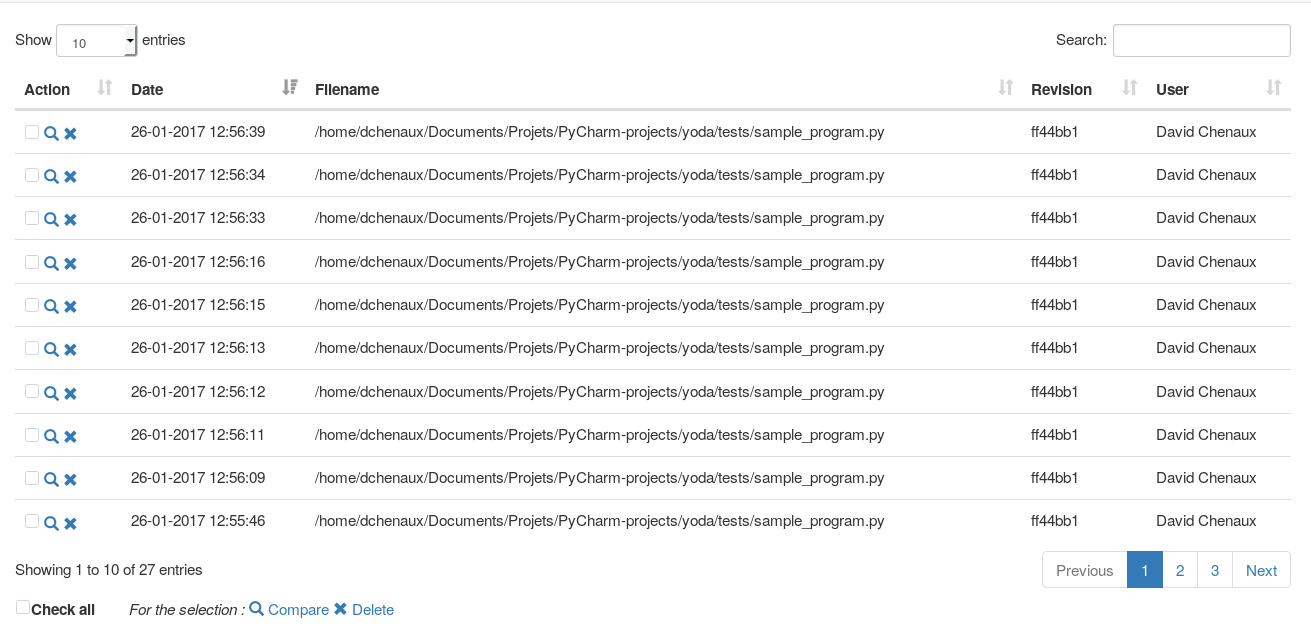
\includegraphics[width=\textwidth]{figures/yoda-home.png}
    \caption{The cockpit}
    \label{fig:home}
\end{figure}

\subsection{The file reviewer}
Once the user selected a run in the cockpit, he will be directly redirected to a reviewing page as illustrated by the \autoref{fig:viewafile}. 
\begin{figure}[h!]
  \centering
    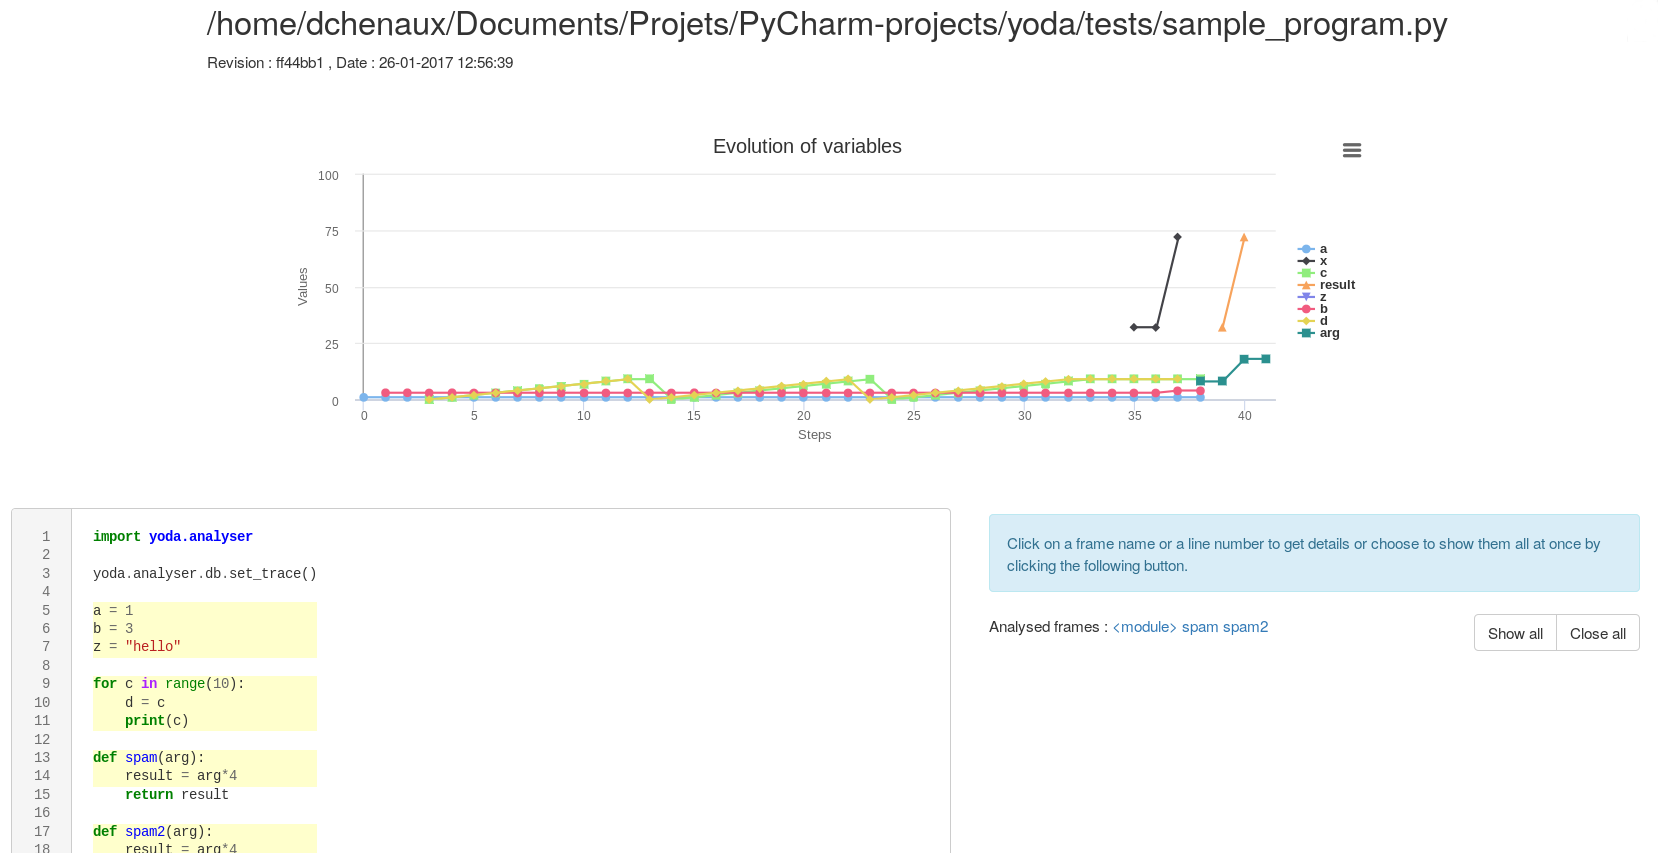
\includegraphics[width=\textwidth]{figures/yoda-file.png}
    \caption{Reviewing a file}
    \label{fig:viewafile}
\end{figure}

This page is separated in 4 main sections. First, at the head of the page the user gets some basic information about the run such as the file name, the date of the run or the git revision. Directly underneath, when possible, a plot graph is computed and shows by default all the available objects. The user can directly from the graph choose to hide some variable and the scope of the graph is automatically adapted to the remaining values. Additionally, the chart can also be printed and exported in several different formats.

A bit further, separated in two vertical columns, the user will find in the left part the complete source code of the analyzed file. The pieces of code which were genuinely analyzed are highlighted in a light yellow color and moreover every line has been numbered and syntactically colored. The line numbers are clickable and open a panel in the left column with some further information about the analyzed objects. Each panel contains a header with the frames name and the line number, and a body with the objects names, their values and a small inline graph resuming the evolution of the value. The \autoref{fig:filefocus} shows in detail these described features. Additionally on the top of the right column some buttons allow to show all the panel, close them or selectively open all panels linked to a frame.

\begin{figure}[h!]
  \centering
    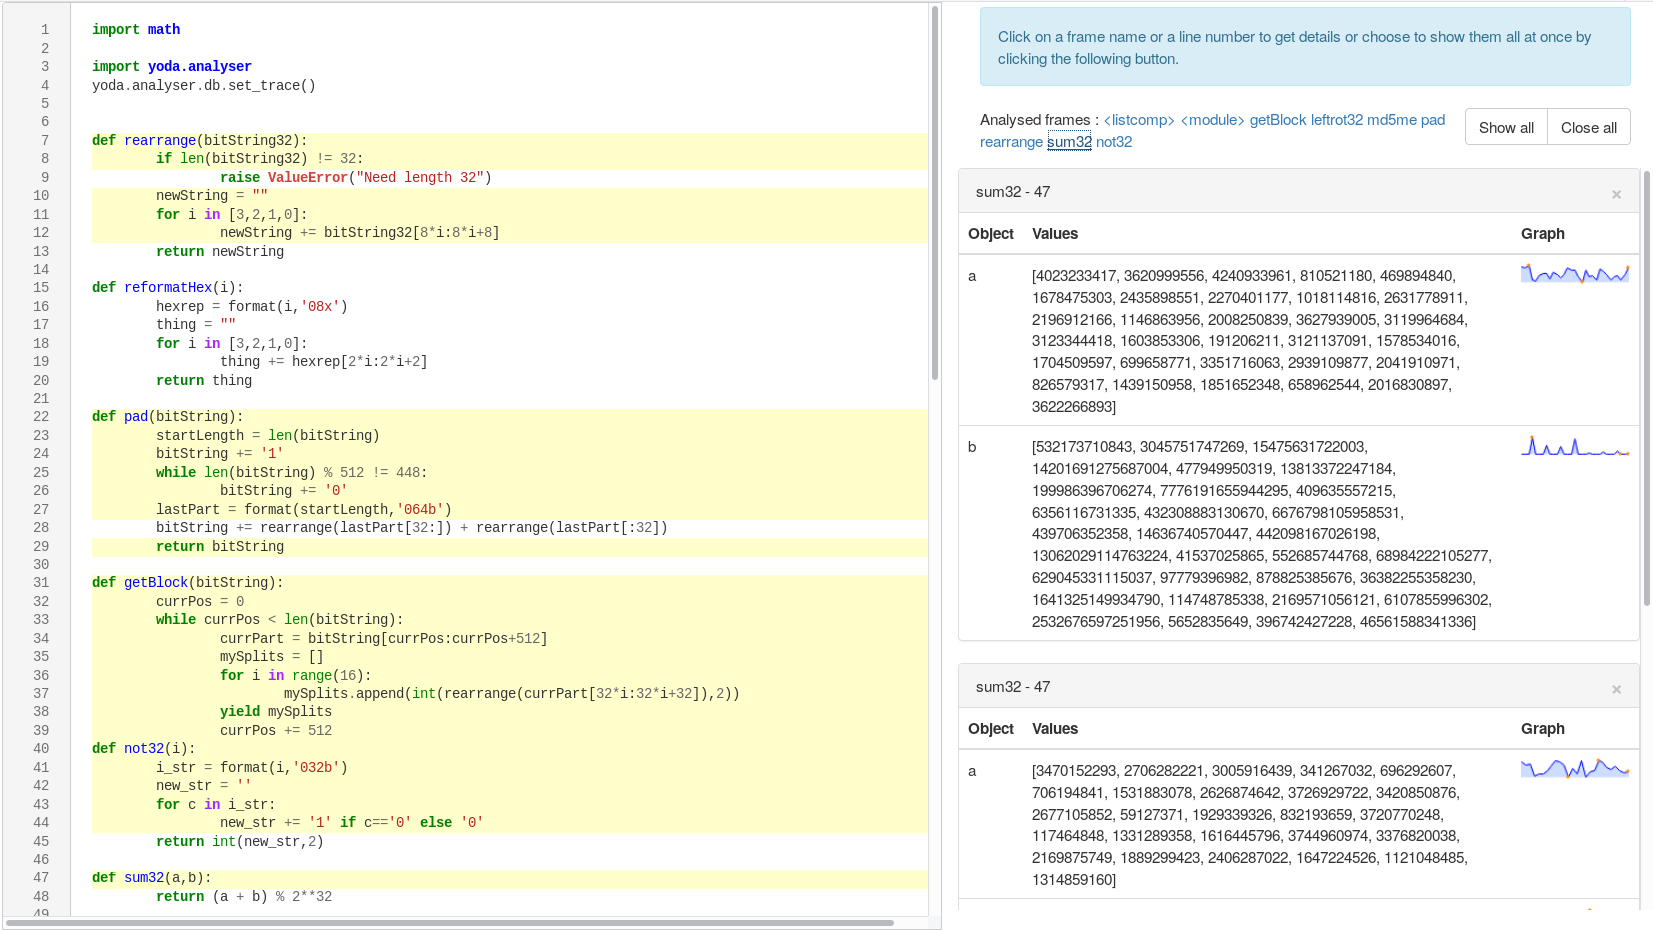
\includegraphics[width=\textwidth]{figures/yoda-file-focus.png}
    \caption{Sources code and detail panels}
    \label{fig:filefocus}
\end{figure}

\subsection{File comparison}
If needed the user has also the possibility to select several files in the cockpit in order to compare them. This is done by checking the needed runs and clicking the "compare" link at the bottom of the page. Doing so will redirect the user on the start page of the comparison. From this page, each file can be inspected and the user is given the choice of which object he wants to select for the comparison as shown on the \autoref{fig:comparisonstart}.
\begin{figure}[h!]
  \centering
    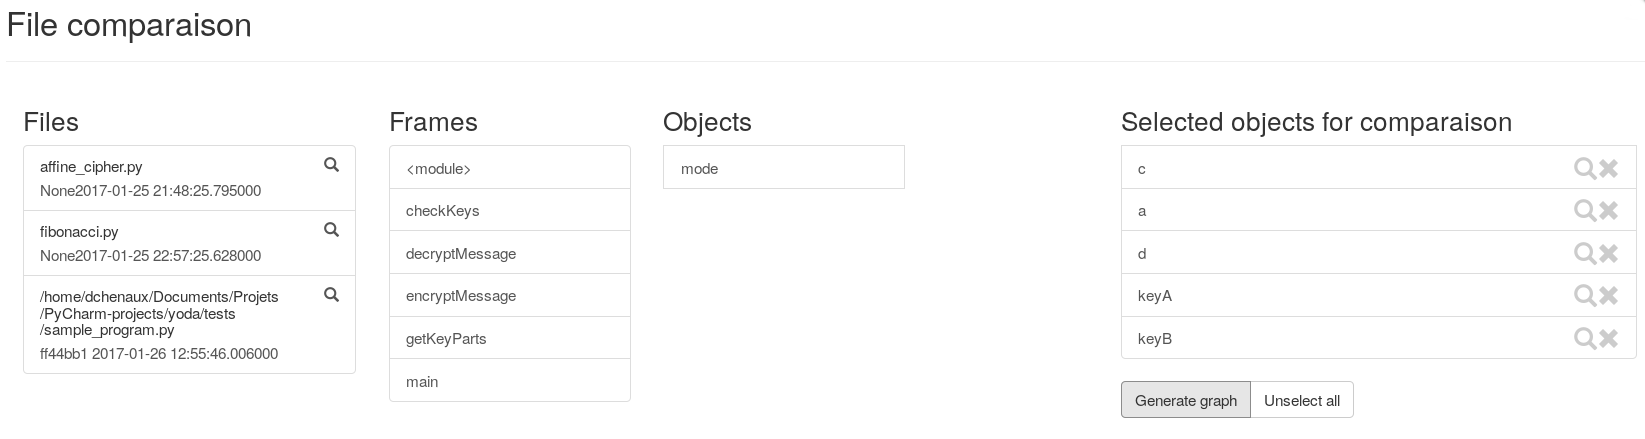
\includegraphics[width=\textwidth]{figures/yoda-comparison.png}
    \caption{Runs comparison}
    \label{fig:comparisonstart}
\end{figure}

For each selected object, the user has the possibility to see the source file or eventually to deselect it. When he is happy with his selection, graphs can be generated with the triggering of the "Generate graphs" button. For each run a graph will be created an disposed in a way which facilitates comparison as shown on \autoref{fig:generatedgraphs}.
\begin{figure}[h!]
  \centering
    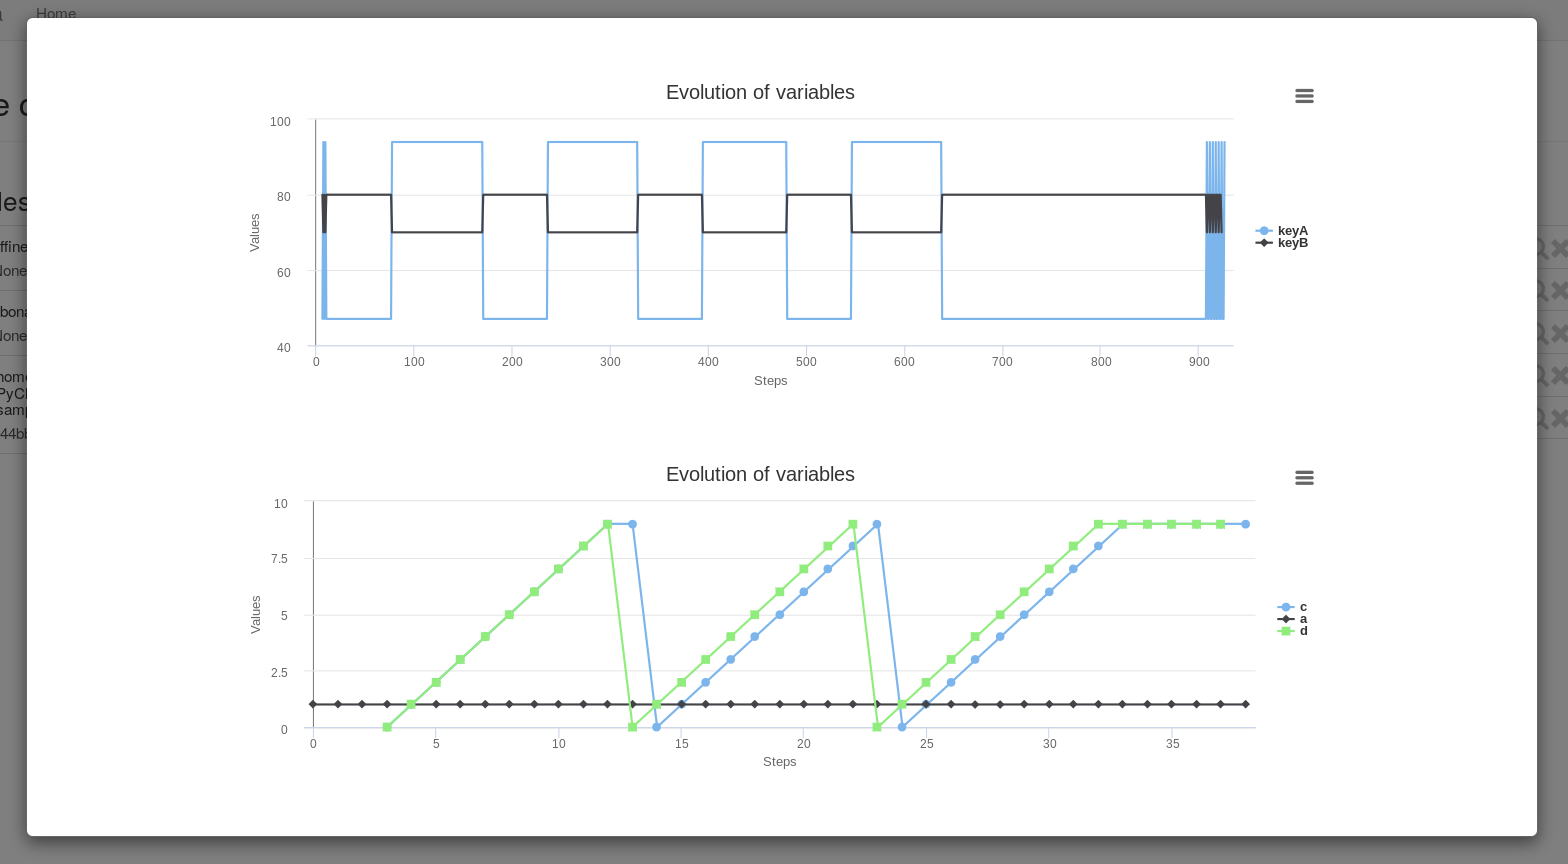
\includegraphics[width=\textwidth]{figures/yoda-graphs.png}
    \caption{Generated graphs for comparison}
    \label{fig:generatedgraphs}
\end{figure}

\section{Concluding remarks}
In this chapter, we tried to give an brief but complete insight of the implementation of our solution. It was quite a challenge to summaries 6 months of development, over 2000 lines of code (around 32'000 with all libraries included !) in a short and comprehensive chapter. The use of Python was a new challenge for us as we were more used to develop in PHP for this kind of application and therefore we has to learn to know and use all the different libraries. The choice of MongoDB was also a discovery as we were more used to work with relation databases. We hope we were able to give the reader a good insight of operating method of our developed system. In the next chapter, we are giving a complete guide to install and start the system.
